\subsection{Sokol}
\begin{wrapfigure}{R}{0.5\textwidth}
  \begin{center}
    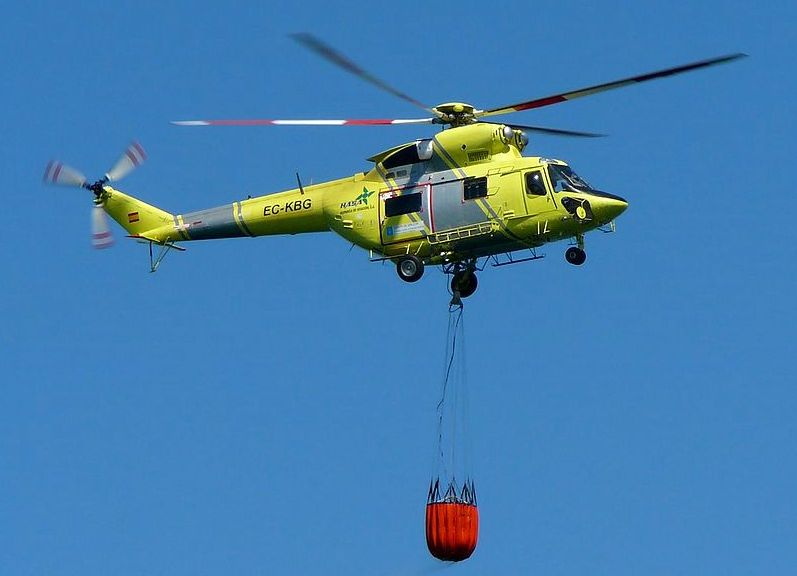
\includegraphics[width=0.35\textwidth]{images/sokol.jpg}
  \end{center}
  \caption{Ejemplo imagen a la derecha}
\end{wrapfigure}
El PZL W-3 Sokół (en polaco significa halcón) es un helicóptero utilitario medio de origen polaco. Se trata de un aparato bimotor de dos plazas que cuenta con un rotor principal de cuatro palas y otro de cola de tres palas. Tiene versiones diseñadas para misiones de transporte de personas y carga, también para asalto aéreo, búsqueda y rescate, SAR y de ataque. 
\subsubsection{Desarrollo}
El W-3 Sokol ('halcón') es el primer helicóptero totalmente diseñado y construido en serie en Polonia. En 1970, Polonia y la URSS firmaron un acuerdo de cooperación para la construcción y el desarrollo de un helicóptero polivalente. El proyecto fue iniciado por la empresa WSK PZL Świdnik en 1973 bajo la dirección de Stanisław Kamiński. En 1976 estuvo listo el primer prototipo y el Sokol hizo su primer vuelo el 16 de noviembre de 1979. Desde entonces ha sido certificado en Polonia, Rusia, EE. UU. y Alemania. Después de un programa de desarrollo bastante prolongado, la producción comenzó durante 1985 en cantidades limitadas. Las primeras ventas del Sokół multipropósito fueron a Polonia y al Bloque del Este antes de la caída del comunismo, lo que permitió a PZL Swidnik ampliar su base de ventas. Con la disolución del Pacto de Varsovia PZL se abrió a Occidente y en 1989 se inició la construcción de una nueva variante. Para ello desarrolló el mejorado Swidnik PZL Sokol W3A encaminado a lograr certificación occidental. La certificación bajo la norma FAR Pt 29 norteamericana se concedió en mayo de 1993, mientras que la certificación alemana fue concedida en diciembre de ese año. El 30 de julio de 1992 lanzó su primer vuelo la producción actual de la variante civil. También se exporta una versión militar.


La versión actual del PZL W-3A2, que recibió la aprobación de Polonia en el 7 de marzo de 2003, cuenta con un sistema electrónico de vuelo EFIS, es decir, un piloto automático de cuatro ejes que junto con el GPS realiza la ubicación y traza una ruta de vuelo de forma autónoma. Además, para las tareas de rescate y transporte, es posible emplear vuelo automático hasta el sitio.


El Sokol es un diseño y construcción convencional, con dos turboejes PZL-10W, que se basan en el PZL-10S versión con licencia de las turbohélices TVD-10B de diseño ruso que potencian el An-28 de construcción polaca también bajo licencia. Materiales compuestos son utilizados en las tres palas del rotor de cola y en las cuatro palas del rotor principal.


El Sokol se ofrece en una serie de variantes y es capaz de realizar un rango de misiones típicas de helicópteros, incluido el transporte de pasajeros, transporte VIP, de carga, EMS (servicios médicos de emergencia de algunos países), evacuación médica, extinción de incendios además de búsqueda y rescate.


La máquina es operada en su versión tanto civil como militar en Chequia, Alemania, España, Birmania, Chile ( Conaf Corporación Nacional Forestal), Polonia (Sily Powietrzne Rzeczypospolitej Polskiej), Portugal, Corea del Sur, Rusia y los Emiratos Árabes Unidos. Hasta 13 de septiembre de 2005 se han construido un total de 146 máquinas completas y cinco de las cabinas en ocho series del PZL W-3. 
\subsubsection{Historia operacional}
Desde 2003 cuatro PZL W-3WA fueron operados por el Grupo Independiente de Ataque Aéreo (Grupa Samodzielna Powietrzno-Szturmowa en polaco) de las fuerzas polacas en Irak. Uno de ellos (número de serie 360902) se estrelló en un accidente cerca de Kerbala, el 15 de diciembre de 2004. Tres soldados murieron y otros tres resultaron heridos.2​


El 3 de abril de 2015 en Nijar (Almería) aparece volcado una de las variantes de carga pintada de amarillo y matrícula EC-KIR, utilizada hasta el verano de 2014 en la lucha contra incendios. Las autoridades investigan cómo ha podido aparecer allí, en la zona no se ha localizado ni a pasajeros, carga o pilotos.
